\subsection{污泥浓缩脱水}
加压溶气气浮法是一种广泛适用于处理不同水量、高浓度悬浮性污染物、油类、微生物、纸浆和纤维的先进处理方法。它已经在城镇污水处理厂中得到广泛应用,并且该工艺在工程实践中已经积累了丰富的经验。

该方法具有多项优势,包括高负荷率、卓越的处理效果和强大的处理能力,能够实现全自动连续运行。此外,通过灵活采用全溶气或部分回流溶气的方式,它还能够适应不同悬浮物浓度的废水处理需求。同时,该技术还能够有效地降低泥渣含水率,保证出水水质的优良。\cite{HJ2007-2010}

因此,在本次污泥浓缩设计中,我们选择了加压溶气气浮法作为处理方法,同时严格遵循中华人民共和国环境保护部《污水气浮处理工程技术规范》(HJ 2007-2010)的要求,以确保设计方案的科学性和可靠性。

\begin{figure}[H]
	\centering
	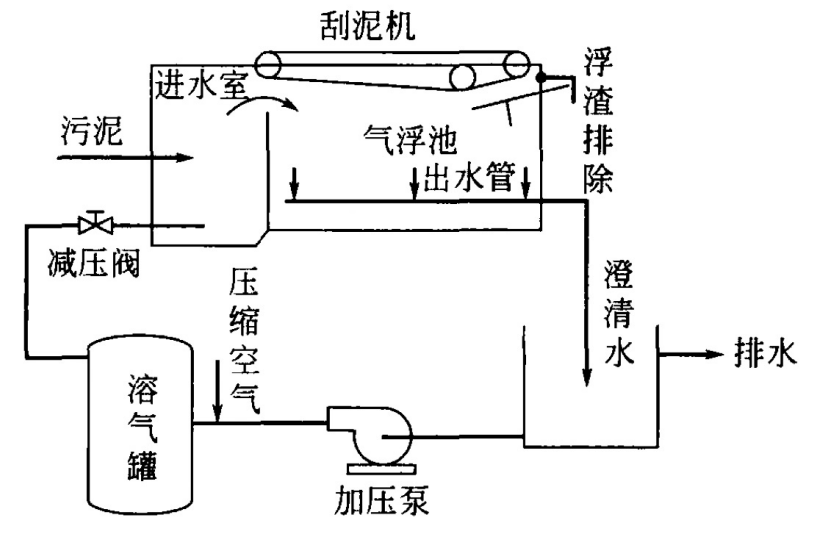
\includegraphics[width=0.8\textwidth]{figures/Sludge thickening process diagram.png}
	\caption{污泥浓缩流程简图}
	\label{fig:Sludge thickening process diagram}
\end{figure}


\subsubsection{基础数据}
% 回流溶气水的回流比(或溶气水比)应计算确定,一般为 $15\%\sim30\%$。\cite{HJ2007-2010}
% 查阅《室外排水设计标准》(GB 50014-2021),由生物反应池后二次沉淀池进入污泥浓缩池的污泥含水率为 $99.2\%\sim 99.6\%$ 时,浓缩后污泥含水率可为 $97.0\%\sim98.0\%$。
% 则数据汇总如下:
\begin{enumerate}
	\item 加压溶气气浮处理工艺中水温控制在20℃;
	\item 剩余污泥量 $\Delta X=5670$ kg/d (计算见公式 \ref{eq:Amount of sludge remaining} );
	\item 污水中悬浮物质量浓度,$S_a=2.6$ kg/m$^3$;
	\item 溶气罐设计工作压力一般为 $0.4\sim0.5$ MPa\cite{HJ2007-2010},则溶气压力取 $P=0.4 \;\text{MPa}=3.95 \;\text{atm}$;
	% \item 设进⼊污泥浓缩池的污泥含⽔率为 $99.6\%$;
	\item 回流溶气水的回流比或溶气水比(一般为 $15\%\sim30\%$\cite{HJ2007-2010}),$R =30 \%$。
	% \item 气固比 $\alpha$ 与悬浮颗粒的疏水性有关,一般情况下 $\alpha=0.005\sim 0.006$,通常由试验确定。% 在这里取 $\alpha=0.005$。
\end{enumerate}
因为气浮池的数量为2,则单个气浮池的剩余污泥流量 $Q$ 为
\begin{align}
	Q=\dfrac{\Delta X}{S_a}=\dfrac{5670}{2.6 \times 24 \times 2} \;\text{m$^3$/h} = \eval{\dfrac{5670}{2.6 \times 24 \times 2}}[3] \;\text{m$^3$/h}
\end{align}


\subsubsection{加压溶气气浮工艺指标计算}
\begin{enumerate}
	\item 气浮某种物质的气固比 $\alpha$
	
	\begin{equation}
		\alpha = \dfrac{\gamma C_s(fP-1)R}{S_a}
	\end{equation}
	$\alpha$——气浮某种物质的气固比;\par
	$\gamma$——空气容重,gL,见表 \ref{tab:The solubility of air in water};\par
	$C_s$——在一定温度下,一个大气压时的空气溶解度,mL/L $\cdot$ atm,见表 \ref{tab:The solubility of air in water};\par
	$f$——加压溶气系统的溶气效率,$f=0.8\sim0.9$;\par
	$P$——溶气压力,绝对压力,atm;\par
	$R$——试验条件下回流比或溶气水回流比,\%;\par
	$S_a$——污水中悬浮物质量浓度,kg/m$^3$;\par

	\begin{table}[H]
		\centering
		\caption{空气在水中的溶解度}
		\begin{tabular}{ccc}
		\toprule
		温度/℃  & 空气容重$\gamma$/(g/L) & 空气溶解度$C_s$(mL/L $\cdot$ atm) \\
		\midrule
		0     & 1.252 & 29.2 \\
		10    & 1.206 & 22.8 \\
		20    & 1.164 & 18.7 \\
		30    & 1.127 & 15.7 \\
		40    & 1.092 & 14.2 \\
		\bottomrule
		\end{tabular}%
		\label{tab:The solubility of air in water}%
	\end{table}%

	因为空气温度一般在20℃左右,所以空气容重取 $\gamma=1.164$ g/L,空气溶解度取 $C_s=18.7$ mL/L $\cdot$ atm,加压溶气系统的溶气效率取 $f=0.8$,则气浮某种物质的气固比 $\alpha$ 为
	\begin{align*}
		\alpha = \dfrac{\gamma C_s(fP-1)R}{S_a} &= \dfrac{1.164 \times 18.7\times (0.8 \times 3.95-1)\times 30\%}{2.6 \times 1000} \\
		&= \eval{\dfrac{1.164 \times 18.7\times (0.8 \times 3.95-1)\times 0.30}{2.6 \times 1000}}[4] \quad\text{(在 $0.005\sim 0.006$ 之间,满足条件)}
	\end{align*}

	\item 气浮池所需空气量 $Q_g$
	
	\begin{equation}\label{eq:alpga to Qg}
		\alpha = \dfrac{Q_g}{Q S_a}
	\end{equation}
	$Q_g$——气浮池所需空气量,kg/h;\par
	$Q$——气浮池处理水量,m$^3$/h; \par
	由上式 \ref{eq:alpga to Qg} 气固比 $\alpha$ 计算公式得,可以反向求出气浮池所需空气量 $Q_g$ 为
	\begin{align*}
		Q_g = \alpha Q S_a &= 0.0054 \times 45.433 \times 2.6 \;\text{kg/h} \\
		&= \eval{0.0054 \times 45.433 \times 2.6}[4] \;\text{kg/h}
	\end{align*}

	\item 所需空压机额定气量 $Q_g'$
	
	\begin{equation}
		Q_g'=\dfrac{\varPsi' Q_g}{60\gamma}
	\end{equation}
	$Q_g'$——所需空压机额定气量,m$^3$/min;\par
	$\varPsi'$——安全系数,$1.2\sim 1.5$。

	取安全系数 $\varPsi'=1.5$,则带入求得
	\begin{align*}
		Q_g'=\dfrac{\varPsi' Q_g}{60\gamma} &=\dfrac{1.5\times 0.6379}{60\times 1.164} \;\text{m$^3$/min} = \eval{\dfrac{1.5\times 0.6379}{60\times 1.164}}[4] \;\text{m$^3$/min}
	\end{align*}

	\item 溶气水量 $Q_r$
	
	\begin{equation} \label{eq:Reflux ratio R}
		R=\dfrac{Q_r}{Q}=\dfrac{1000\alpha S_a}{\gamma C_s(fP-1)}
	\end{equation}
	$Q_r$——溶气水量,m$^3$/h;\par

	由回流比 $R$ 计算公式 \ref{eq:Reflux ratio R} 得:
	\begin{equation}
		Q_r=QR = 45.433\times 30\% \;\text{m$^3$/h} = \eval{45.433\times 30/100}[3] \;\text{m$^3$/h}
	\end{equation}
\end{enumerate}


% \subsubsection{加压溶气气浮工艺指标计算 old}
% \begin{enumerate}
% 	\item 气浮池所需空气量 $Q_g$
	
% 	\begin{equation}
% 		Q_g=\dfrac{\gamma C_s(fP-1)RQ}{1000}
% 	\end{equation}
% 	$Q_g$——气浮池所需空气量,kg/h;\par
% 	$\gamma$——空气容重,gL,见表 \ref{tab:The solubility of air in water};\par
% 	$Q$——气浮池处理水量,m$^3$/h; \par
% 	$R$——试验条件下回流比或溶气水回流比,\%;\par
% 	$C_s$——在一定温度下,一个大气压时的空气溶解度,mL/L $\cdot$ atm,见表 \ref{tab:The solubility of air in water};\par
% 	$P$——溶气压力,绝对压力,atm;\par
% 	$f$——加压溶气系统的溶气效率,$f=0.8\sim0.9$。\par

	

% 	因为空气温度一般在20℃左右,所以空气容重取 $\gamma=1.164$ gL,空气溶解度取 $C_s=18.7$ mL/L $\cdot$ atm,加压溶气系统的溶气效率取 $f=0.8$,又因为回流比 $R$
% 	\begin{equation} \label{eq:Reflux ratio R}
% 		R=\dfrac{Q_r}{Q}=\dfrac{1000\alpha S_a}{\gamma C_s(fP-1)}
% 	\end{equation}
% 	$Q_r$——溶气水量,m$^3$/h;\par
% 	$S_a$——污水中悬浮物质量浓度,kg/m$^3$;\par
% 	$\alpha$——气浮某种物质的气固比。

% 	则
% 	\begin{align*}
% 		R =\dfrac{Q_r}{Q} =\dfrac{1000\alpha S_a}{\gamma C_s(fP-1)} &= \dfrac{1000\times 0.005\times 2.8}{1.164\times 18.7\times(0.8\times 3.95-1)} \\
% 		&= \eval{\dfrac{1000\times 0.005\times 2.8}{1.164\times 18.7\times(0.8\times 3.95-1)}}  \\
% 		& \approx 30 \;\text{\%(向上取整)}
% 	\end{align*}
% 	% 效验结果:根据《污水气浮处理工程技术规范》(HJ 2007-2010),回流溶气水的回流比(或溶气水比)应计算确定,一般为 $15\%\sim30\%$。符合要求。

% 	所以气浮池所需空气量 $Q_g$ 为
% 	\begin{align*}
% 		Q_g=\dfrac{\gamma C_s(fP-1)RQ}{1000} &=\dfrac{1.164\times 18.7\times(0.8\times 3.95-1)\times 30\%\times 117.42}{1000} \;\text{kg/h} \\
% 		&= \eval{\dfrac{1.164\times 18.7\times(0.8\times 3.95-1)\times 30/100 \times 117.42}{1000}}[3] \;\text{kg/h}
% 	\end{align*}

% 	% \item 气浮某种物质的气固比 $\alpha$ 
	
% 	% 气固比 $\alpha$ 与悬浮颗粒的疏水性有关,$\alpha=0.005\sim 0.006$,通常由试验确定。当无资料时,可按下式计算:
% 	% \begin{align}
% 	% 	\alpha &=\dfrac{Q_g}{QS_a}=\dfrac{\gamma C_s(fP-1)R}{1000S_a}
% 	% 	% & =\dfrac{1.656}{117.42\times 0.005} \;\text{kg/m$^3$} \notag \\
% 	% 	% & =\eval{\dfrac{1.656}{117.42\times 0.005}}[4] \;\text{kg/m$^3$} \notag 
% 	% \end{align}
% 	% $S_a$——污水中悬浮物质量浓度,kg/m$^3$。

% 	\item 所需空压机额定气量 $Q_g'$
	
% 	\begin{equation}
% 		Q_g'=\dfrac{\varPsi' Q_g}{60\gamma}
% 	\end{equation}
% 	$Q_g'$——所需空压机额定气量,m$^3$/min;\par
% 	$\varPsi'$——安全系数,$1.2\sim 1.5$。

% 	取安全系数 $\varPsi'=1.5$,则带入求得
% 	\begin{align*}
% 		Q_g'=\dfrac{\varPsi' Q_g}{60\gamma} =\dfrac{1.5\times 1.656}{60\times 1.164} \;\text{m$^3$/min} = \eval{\dfrac{1.5\times 1.656}{60\times 1.164}}[4] \;\text{m$^3$/min}
% 	\end{align*}

% 	\item 溶气水量 $Q_r$

% 	\begin{equation}
% 		Q_r=\dfrac{Q_g}{736fPK_T}
% 	\end{equation}
% 	$f$——溶气效率,对装阶梯环填料的溶气罐可取0.9;\par
% 	$P$——选定的溶气压力,atm;\par
% 	$K_T$——溶解度系数,可根据水温查表 \ref{tab:KT values at different temperatures} 而得。

% 	\begin{table}[H]
% 		\centering
% 		\caption{不同温度下的$K_T$值}
% 		\begin{tabular}{ccccccc}
% 		\toprule
% 		温度/℃  & 0     & 10    & 20    & 30    & 40    & 50 \\
% 		\midrule
% 		$K_T$值    & 0.038 & 0.029 & 0.024 & 0.021 & 0.018 & 0.016 \\
% 		\bottomrule
% 		\end{tabular}%
% 		\label{tab:KT values at different temperatures}%
% 	\end{table}%

% 	因为温度为20℃,所以溶解度系数 $K_T=0.024$,则溶气水量 $Q_r$ 为
% 	\begin{align*}
% 		Q_r=\dfrac{Q_g}{736fPK_T}=\dfrac{1.656}{736\times 0.8\times 3.95\times 0.024} \;\text{m$^3$/h} =\eval{\dfrac{1.656}{736\times 0.8\times 3.95\times 0.024}}[4] \;\text{m$^3$/h}
% 	\end{align*}

% 	由回流比 $R$ 计算公式 \ref{eq:Reflux ratio R} 得:
% 	\begin{equation}
% 		Q_r=QR = 117.42\times 30\% \;\text{m$^3$/h} = \eval{117.42\times 30/100} \;\text{m$^3$/h}
% 	\end{equation}
% \end{enumerate}


\subsubsection{气浮池接触室}
\begin{enumerate}
	\item 接触室表面积 $A_c$
	
	\begin{equation}
		A_c=\dfrac{Q+Q_r}{3600v_c}
	\end{equation}
	$A_c$——接触室表面积,m$^3$;\par
	$v_c$——水流平均速度,通常取 $10\sim20$ mm/s.

	取水流平均速度 $v_c=10 \;\text{mm/s} =0.01 \;\text{m/s}$,则接触室表面积 $A_c$ 为
	\begin{align*}
		A_c=\dfrac{Q+Q_r}{3600v_c}=\dfrac{45.433+13.63}{3600\times0.01} \;\text{m$^2$} = \eval{\dfrac{45.433+13.63}{3600\times0.01}}[4] \;\text{m$^2$}
	\end{align*}

	\item 接触室长度 $L$
	
	\begin{equation}
		L=\dfrac{A_c}{B_c}
	\end{equation}
	$L$——接触室长度,m;\par
	$B_c$——接触室宽度,m。

	因为平流式长宽比一般为 $2:1\sim3:1$\cite{HJ2007-2010},所以令 $L=2B_c$,则
	\begin{align*}
		L=\sqrt{2A_c} &=\sqrt{2\times 1.6406} \;\text{m} = \eval{\sqrt{2\times 1.6406}} \;\text{m} \\
		& \approx 1.82 \;\text{m(向上保留2位小数)}
	\end{align*}
	所以 $B_c=L/2=0.91$ m。

	\item 接触室堰上水深 $H_2$
	
	\begin{equation}
		H_2=B_c=0.91 \;\text{m}
	\end{equation}

	\item 接触室气水接触时间 $t_c$
	
	\begin{equation}
		t_c=\dfrac{H_1-H_2}{v_c}
	\end{equation}
	$t_c$——接触室气水接触时间,要求 $t_c>60$ s;\par
	$H_1$——气浮池分离室水深,通常为 $1.8\sim2.2$ m。

	取气浮池分离室水深 $H_1=1.8$ m,则
	\begin{align*}
		t_c=\dfrac{H_1-H_2}{v_c}=\dfrac{1.8-0.91}{0.01} \;\text{s} = \eval{\dfrac{1.8-0.91}{0.01}} \;\text{s($> 60$ s,满足要求)}
	\end{align*}
\end{enumerate}


\subsubsection{气浮分离室}
\begin{enumerate}
	\item 分离室表面积 $A_s$
	
	\begin{equation}
		A_s=\dfrac{Q+Q_r}{3600v_s}
	\end{equation}
	$A_s$——分离室表面积,m$^2$;\par
	$v_s$——分离室水流向下平均速度,通常为 $1\sim1.5$ mm/s。

	取分离室水流向下平均速度 $v_s=1.5$ mm/s,则分离室表面积 $A_s$ 为
	\begin{align*}
		A_s=\dfrac{Q+Q_r}{3600v_s} = \dfrac{45.433 + 13.63}{3600\times 1.5\times 10^{-3}} \;\text{m$^2$} = \eval{\dfrac{45.433 + 13.63}{3600\times 1.5\times 10^{-3}}}[3] \;\text{m$^2$}
	\end{align*}

	\item 分离室长度 $L_s$
	
	\begin{equation}
		L_s=\dfrac{A_s}{B_s}
	\end{equation}
	$L_s$——分离室长度,m;\par
	$B_s$——分离室宽度,m。

	因为对矩形池,分离室的长宽比一般取 $2:1\sim3:1$,所以令$L_s=2B_s$,则
	\begin{align*}
		L_s=\sqrt{2A_s} &=\sqrt{2\times 10.938} \;\text{m} = \eval{\sqrt{2\times 10.938}} \;\text{m} \\
		& \approx 4.68 \;\text{m(向上保留2位小数)}
	\end{align*}
	所以 $B_c=L/2=2.34$ m。

	\item 气浮池水深 $H$
	
	\begin{equation}
		H=v_s t
	\end{equation}
	$H$——气浮池水深,m;\par
	$t$——气浮池分离室停留时间,一般取 $10\sim 20$ min。

	取气浮池分离室停留时间 $t=20$ min,则气浮池水深 $H$ 为
	\begin{align*}
		H=v_s t=1.5 \times 10^{-3} \times 20 \times 60 \;\text{m} = \eval{1.5 \times 10^{-3} \times 20 \times 60} \;\text{m}
	\end{align*}

	\item 气浮池容积 $W$
	
	\begin{align}
		W= (A_c+A_s)\cdot H = (1.6406+10.938)\times 1.8 \;\text{m$^3$} = \eval{(1.6406+10.938)\times 1.8}[3] \;\text{m$^3$}
	\end{align}

	\item 总停留时间 $T$ 校核
	
	\begin{align}
		T=\dfrac{60\times W}{Q+Q_r} &= \dfrac{60\times 22.641}{45.433 + 13.63} \;\text{min} = \eval{\dfrac{60\times 22.641}{45.433 + 13.63}} \;\text{min} \\
		&\approx 23 \;\text{min} \notag
	\end{align}
\end{enumerate}


% \subsubsection{水位控制室}
% 水位控制室宽度 $B$ 不小于 900 mm,以便安装水位调节器,并利于检修。水位控制室可设于分离室一端,其长度等于分离室宽度。水位控制室深度一般与气浮分离室同深。


\subsubsection{溶气设备}
溶气罐应设安全阀,顶部最高点应装排气阀。溶气水泵进入溶气罐的入口管道应设除污过滤器。溶气罐底部应装快速排污阀。

溶气罐应设水位、压力仪表及自控装置。
\begin{enumerate}
	\item 压力溶气罐直径 $D_d$
	
	\begin{equation}
		D_d=\sqrt{\dfrac{4\times Q_r}{\pi I}}
	\end{equation}
	$D_d$——压力溶气罐直径,m;\par
	$I$——单位罐截面积的水力负荷,m;一般为 $80\sim 150$ m$^3$/(m$^2 \cdot$h),填料罐选用 $100\sim200$ m$^3$/(m$^2 \cdot$h)。

	取单位罐截面积的水力负荷 $I=80$ m$^3$/(m$^2 \cdot$h),如果只用1个溶气罐给2个池子充气,则压力溶气罐直径 $D_d$ 为
	\begin{align*}
		D_d=\sqrt{\dfrac{4\times Q_r}{\pi I}} &= \sqrt{\dfrac{4\times 13.63 \times 2}{\pi \times 80}} \;\text{m} = \eval{\sqrt{\dfrac{4\times 13.63\times 2}{\pi \times 80}}} \;\text{m} \\
		& \approx 750 \;\text{mm(向上取整)}
	\end{align*}

	\item 溶气罐高度 $Z$
	
	根据《污水气浮处理工程技术规范》(HJ 2007-2010),溶气罐一般为立式,设计高径比应大于 $2.5\sim 4$,有条件时取高值。则设计溶气罐高径比 $Z/D_d=4$,那么溶气罐高度 $Z$ 为
	\begin{equation}
		Z = 4 D_d = 4\times 0.750 \;\text{m} = 3.0 \;\text{m}
	\end{equation}
	又因为溶气罐高度 $Z$ 还可以通过下列公式计算:
	\begin{equation}
		Z = 2Z_1 + Z_2 + Z_3 + Z_4
	\end{equation}
	$Z$——溶气罐高度,m;\par
	$Z_1$——罐顶、底封头高度,m(根据罐直径而定);\par
	$Z_2$——布水区高度,一般取 $0.2\sim 0.3$ m;\par
	$Z_3$——贮水区高度,一般取 1.0 m;\par
	$Z_4$——填料层高度,当采用阶梯环时,可取 $1.0\sim 1.3$ m。

	溶气罐必要时可装填料,一般采用阶梯环填料,填料层高度应为罐高的 1/2,并不少于 0.8 m,液位控制高为罐高的 $1/4\sim 1/2$(从罐底计)\cite{HJ2007-2010}。所以取 $Z_2=0.3$ m,$Z_3=1.0$ m,$Z_4=Z/2 = 1.5$ m,则可以反求出罐顶、底封头高度 $Z_1$ 为
	\begin{align*}
		Z_1 = \dfrac{Z -(Z_2 + Z_3 + Z_4)}{2} &= \dfrac{3.0 -(0.3 + 1.0 + 1.5)}{2} \;\text{m} \\
		&= \eval{\dfrac{3.0 -(0.3 + 1.0 + 1.5)}{2}} \;\text{m}
	\end{align*}
	% 所以 $Z_4 = \dfrac{1}{2}Z = 1.4$ m $>0.8$ m(符合要求)。

	\item 溶气罐体积 $V_d$ 复核
	
	溶气罐水力停留时间 $t_d$ 应大于 $2 \sim 3$ min(有填料时取低值),并应计算确定;
	溶气水在溶气罐内停留时间:当无填料时 $t_d = 3\sim 3.5$ min;当有填料时 $t_d =2$ min。

	$\bullet $ 实际溶气罐体积
	\begin{align}
		V_d = \dfrac{\pi D_d^2}{4} \cdot Z = \dfrac{\pi \times 0.750^2}{4} \times 3.0 \;\text{m$^3$} = \eval{\dfrac{\pi \times 0.750^2}{4} \times 3.0}[3] \;\text{m$^3$}
	\end{align}
	$\bullet $ 理论溶气罐体积(用1个溶气罐给2个池子充气,取 $t_d =2$ min)
	\begin{align}
		V_d = Q_r \cdot t_d = \dfrac{13.63 \times 2 \times 2}{60} \;\text{m$^3$} = \eval{\dfrac{13.63 \times 2 \times 2}{60}}[3] \;\text{m$^3$}
	\end{align}

	% \item 溶气罐高径比 $Z/D_d$ 复核
	
	% 根据《污水气浮处理工程技术规范》(HJ 2007-2010),溶气罐一般为立式,设计高径比应大于 $2.5\sim 4$,有条件时取高值。
	
	% \begin{equation}
	% 	\dfrac{Z}{D_d} = \dfrac{3.0}{0.750} = \eval{\dfrac{3.0}{0.750}} \quad\text{(符合标准)}
	% \end{equation}
\end{enumerate}


% \subsubsection{气浮池集水管、集渣槽}
% \begin{enumerate}
% 	\item 气浮池集水管
	
% 	采用穿孔管,按分配流量及流速0.4~0.5 m/s确定管径。并令孔眼水头损失h=0.3 m,计算出孔口流速vo、孔眼尺寸和个数。
	
% 	\begin{equation}
% 		v_0 = \mu \sqrt{2gh}
% 	\end{equation}
% 	$v_0$——孔眼流速,m/s;\par
% 	$\mu$——孔眼流速系数。

% 	\item 集渣槽
	
% 	集渣槽断面设计可按单位时间的排泥量(包括抬高水位所带出的水量)进行选择。一般不小于200 mm,当浮渣浓度较高时,集渣槽需有足够的坡度倾向排泥口,一般应大于 $0.03\sim 0.05$。当集渣槽长度超过5 m时,应由两端向中间排泥。必要时可辅以冲洗水管。
% \end{enumerate}


% \subsubsection{溶气释放器}
% 溶气释放器可选择TJ型或TV型。溶气释放器个数 $n$ 计算公式如下:

% \begin{equation}
% 	n=\dfrac{Q_r}{q}
% \end{equation}
% $q$——选定溶气压力下单个释放器的出流量,m$^3$/h。

% 溶气水由溶气罐至释放器的管道上应设快开阀。

% 释放器应考虑快速拆卸装置。


% \subsubsection{刮渣机}
% 对于矩形气浮池应采用桥式刮渣机刮渣,跨度宜在 10 m以下,集渣槽的位置可在池的一端或两端;圆形气浮池宜采用行星式刮渣机,其适用范围在直径 $2\sim 10$ m,集渣槽位置可在圆池径向的任何部位。


\subsubsection{污泥脱水}
\paragraph{$\bullet $ 基础条件}~{}\par
污泥脱水设备:污泥真空转鼓过滤脱水机
\begin{enumerate}
    \item 该污水处理厂初沉污泥和剩余活性污泥消化后污泥产量 5636.2 m$^3$/d ;
    \item 污泥含水率 $p_0=99.6\%$ ;
    \item 经絮凝剂调质后,污泥比阻 $y=3\times 10^{11}$ m/kg ;
    \item 选用真空转鼓过滤机,要求脱水泥饼含水率达 80\% ;
    \item 过滤压力 $p=4.5\times 10^4$ N/m ;
    \item 过滤周期 $T=120$ s,泥饼形成时间 $t=36$ s ;
    \item 滤液动力黏度 $\mu =0.001$ N·s/m$^2$ 。
\end{enumerate}


\paragraph{$\bullet $ 设计计算}~{}\par
\begin{enumerate}
    \item 计算过滤产率 $L$ [kg/(m$^2$·s)]
    
    \begin{equation}\label{eq:Calculate filtration yield}
        L = \sqrt{\dfrac{2p \omega m}{\mu \gamma T}}
    \end{equation}
    式中:$m$——过滤机的浸液比,$m=t/T$;
    \newline\phantom{式中:}$\omega$——滤过单位体积的滤液在过滤介质上截留的干固体质量,g/mL,$\omega = \dfrac{C_g C_0}{100(C_g - C_0)}$;
    \newline\phantom{式中:}$C_0$——污泥干固体含量,\%;
    \newline\phantom{式中:}$C_g$——泥饼干固体含量,\%。

    因为 $t=36$ s,则过滤机的浸液比 $m$ 为
    \begin{equation}
        m=t/T = 36/120 = 0.3
    \end{equation}
    因为污泥干固体含量 $C_0=0.4\%$,污饼干固体含量 $C_g=20\%$,则滤过单位体积的滤液在过滤介质上截留的干固体质量 $\omega$ 为
    \begin{align}
        \omega = \dfrac{C_g C_0}{100(C_g - C_0)} &= \dfrac{20 \times 0.4}{100\times (20-0.4)} \;\text{g/mL} = \eval{\dfrac{20 \times 0.4}{100\times (20-0.4)}} \;\text{g/mL} \\
        &= \eval{\dfrac{20 \times 0.4}{100\times (20-0.4)}\times 1000}[3] \;\text{kg/m$^3$} \notag
    \end{align}
    将上述计算数据代入公式 \ref{eq:Calculate filtration yield} 得,计算过滤产率 $L$ 为
    \begin{align*}
        L = \sqrt{\dfrac{2p \omega m}{\mu \gamma T}} &= \sqrt{\dfrac{2 \times 4.5\times 10^{4} \times 4.082 \times 0.3}{0.001 \times 3\times 10^{11} \times 120}} \quad\text{kg/(m$^2$·s)} \\
        &= \eval{\sqrt{\dfrac{2 \times 4.5\times 10^{4} \times 4.082 \times 0.3}{0.001 \times 3\times 10^{11} \times 120}}} \;\;\text{kg/(m$^2$·s)} \notag \\
        &= \eval{\sqrt{\dfrac{2 \times 4.5\times 10^{4} \times 4.082 \times 0.3}{0.001 \times 3\times 10^{11} \times 120}}\times 3600}[2] \;\;\text{kg/(m$^2$·h)} \notag
    \end{align*}

    \item 过滤面积 $A$ (m$^2$)
    
    所需真空过滤机过滤面积为
    \begin{equation}
        A = \dfrac{af(1-p_0)Q\cdot 10^{3}}{L}
    \end{equation}
    式中:$a$——安全系数,取 $a=1.15$;
    \newline\phantom{式中:}$f$——考虑投加混凝剂污泥干重增加系数,取 $f=1.15$;
    \newline\phantom{式中:}$Q$——污泥量,m$^3$/h;
    \newline\phantom{式中:}$p_0$——污泥含水率,\%。

    已知日产污泥量 5636.2 m$^3$/d,脱水机每天工作两班,每班 8 h,则
    \begin{equation}
        \text{每小时污泥量} = \dfrac{5636.2}{2\times 8} \;\text{m$^3$/h} = \eval{\dfrac{5636.2}{2\times 8}}[2] \;\text{m$^3$/h}
    \end{equation}
    所以,过滤面积 $A$ 为
    \begin{align*}
        A = \dfrac{af(1-p_0)Q\cdot 10^{3}}{L} &= \dfrac{1.15\times 1.15\times (1-99.6\%)\times 352.26\times 10^{3}}{6.30} \;\text{m$^2$} \\
        &= \eval{\dfrac{1.15\times 1.15\times (1-0.996)\times 352.26\times 10^{3}}{6.30}}[2] \;\text{m$^2$}
    \end{align*}

    选用 5 台 G80-3.5 型转鼓真空过滤机,其中 1 台备用。每台脱水机过滤面积 80 m$^2$,转鼓直径 3.5 m$^2$,配电功率 5 kW。

    \item 附属设备的选择
    \begin{enumerate}[label=(\arabic*)]
        \item 真空泵。\\
        抽气量按 1 m$^2$ 介质面积 $0.5\sim 1.0$ m$^3$/min 估算,真空度 $200\sim 500$ mmHg (l mmHg $=133.3$ Pa),电机功率按 1 m$^3$/min 配 1.2 kW,则
		\begin{itemize}
			\item 抽气量 $Q = 40 \times 0.6 \;\text{m$^3$/min} = 24 \;\text{m$^3$/min}$
			\item 真空度 500 mmHg = 66661 Pa
			\item $\text{配电功率}=24\times 1.2 \;\text{kW} =28.8 \;\text{kW}$
		\end{itemize}
        故选用 2 台真空泵。

        \item 空压机。\\
        压缩气量按每 1 m$^2$ 介质 0.1 m$^3$/min 估算,压力 $0.2\sim 0.3$ MPa,电机功率按 1 m$^3$/min 配 4 kW 计算,则
		\begin{itemize}
			\item 压缩空气量 $Q=40 \times 0.1 \;\text{m$^3$/min} =4 \;\text{m$^3$/min}$,压力取 0.3 MPa
			\item 配电功率 $=4\times 4 \;\text{kW} =16 \;\text{kW}$
		\end{itemize}
        故空压机设置 2 台。

        \item 反冲洗泵。\\
        冲洗水量按 1 m$^2$ 介质面积 $0.8\sim 1.3$ L/s 计算,水压 $294\sim 343$ kPa ($3\sim 3.5$ kgf/cm$^2$)。
		\begin{itemize}
			\item 冲洗流量 $Q=40 \times 1.0 \;\text{L/s} =40 \;\text{L/s}$
			\item 冲洗水压 $H=343$ kPa (3.5 kgf/cm$^2$)
		\end{itemize}
        故反冲洗泵设置 2 台。
    \end{enumerate}
\end{enumerate}

